\chapter{Evaluation of the Fitting with the Segmentation of the FCN}
The EM-algorithm like method of \cite{egger_paper} uses a binary mask to determine whether a pixel is relevant for the fitting-process or if it's not. We changed the EM-like method of Egger et al. to not estimate a mask at all, but use the same initial mask in each iteration. But we let this EM-algorithm estimate the parameters for a 3DMM (3D Morphable Model) in order to get a 3D reconstruction of the 2D face. As the Morphable Model we use the popular Basel Face Model of 2017 \cite{BFM2017} which was originally proposed in 1999 by Blanz and Vetter \cite{BlanzVetter}. The Parametric-Face-Image-Generator of \cite{parametric} outputs renderings of sample facial images, provides the ground truth parameters of the face and provides a ground truth segmentation. Since we want to measure the fitting accuracy with the masks of Egger itself and the FCN-Segmentation only, we render occlusions over the facial image as in the previous chapter.\\
\\
The experiments in this cchapter will only be explained with one specific type of occlusions (hands) so as not to overwhelm the reader. Of course, we repeated the experiments on all occlusions that the FCN from Nirkin et al. was trained on. Please find these fits and the error-plots in the appendix. \\
\\
The fitting method of Egger et al. is guided by landmarks on the face (eg. nose-tip, mouth-corner). Each landmark has a boolean flag which determines whether the landmark is visible for the observer or not. Because the Parametric-Face-Image-Generator was originally developed to render only a face in a certain pose and without any occlusions, all landmarks were labeled as visible per se. Therefore, we had to turn off those who were covered by an occlusion (see Figures \ref{fig:chap3:lms:1} and \ref{fig:chap3:lms:2}).\\
\\
\begin{figure}
	\hspace*{\fill}%
	\subbottom[A facial image of the Parametric-Face-Image-Generator with all landmarks activated.]{\includegraphics[width=0.3\textwidth]{Figures/chap3/original_all_lms.png}\label{fig:chap3:lms:1}}\hfill
	\subbottom[The same image as in \ref{fig:chap3:lms:1} but with an occlusion and two underlying landmarks which are disabled because they're not visible anymore.]{\includegraphics[width=0.3\textwidth]{Figures/chap3/occluded_parts_lms.png}\label{fig:chap3:lms:2}}
	\hspace*{\fill}%
	\caption{The original landmarks (green dots) and the landmark which had to be disabled because of the occlusion (red dots)}
	\label{fig:chap3:lms}
\end{figure}

For the evaluation of the fitting, we generated faces with 150 parameters. 50 of them were for the shape of the Basel Face Model, another 50 for the color and the last 50 for the expression. We now render different faces with various occlusions, various angles/poses, a random illumination and cover them with different occlusions.\\
\\
The aim of this chapter is to reconstruct the generated synthetic faces with the EM-like algorithm of Egger et al. which estimates fitting parameters and a segmentation itself. But we manipulate the algorithm that it skips the E-step and takes the segmentation of the FCN, the ground truth segmentation or no mask in every iteration. To get acceptable results we fix the number of EM steps to 20. In this experiment, we measure the fitting accuracy and speed, without letting the fitting algorithm produce it's own z-labels. The FCN is trained to cut hands, glasses and microphones out of the picture. That's why in the following experiments we use these three classes of occlusions and test the segmentation of the FCN an a dataset without any occlusions too. With the mask of the FCN, the fitting should also be much faster, because the time-consuming job of updating the z labels is eliminated. After every iteration, we get information about pose, probability of the current fit and about the 3DMM parameters of the fit. We compare those to the ground truth information from the Parametric-Face-Image-Generator. To calculate the error, we use the RMSE (Root Mean Squared Error).\\
\\


\section{Evaluation on a tailored face}
In this setting, we use the 'face12' version of the Basel Face Model. It has in contrast to the original no neck, no ears and no hairline. \Cref{fig:chap3:plot_hands_setup1} shows the error of the parameters, the angles, illumination and the probability in every iteration. The experiments are repeated 10 times with different faces. We see that in all the parameters (shape, color and expression) the quality of the fit with the FCN segmentation is very close to the one of the iterative approach of Egger et al. The differences in the Euler angles (yaw, pitch and roll) are negligible, since all errors move in a very small order. The plot named 'EnvironmentMap' shows the deviation of the illumination parameters.\\
\\
For updating the 3DMM-Parameters in every iteration (M-Step), the algorithm of Egger et al. does a Metropolis-Hastings like Random-Walk in the parameter space. The walk is guided by the probability of the proposal and tries to maximize it. Unfortunately, you can not compare the curves of the last plot (posterior) directly with each other, as the value of the posterior depends very much on the segmentation used. The more pixels are segmented as face, the more terms the evaluator adds to the posterior. Therefore it can vary very strongly. It is added up because the negative logarithm is applied to the probability value for each pixel. $P(\Theta)=\prod_{x_i \in \text{facepixels}}p(x_i ; \Theta) \rightarrow L(\Theta)=\sum_{x_i \in \text{facepixels}}-ln(p(x_i ; \Theta))$. This is valid because the logarithm is a monotonic increasing function.

\begin{figure}
\centering
	\subbottom[original facial image]{\includegraphics[width=.4\textwidth]{Figures/chap3/hands_setting1_original_test6.png}\label{fig:chap3:hands_original}}\qquad
	\subbottom[facial image with occlusion]{\includegraphics[width=.4\textwidth]{Figures/chap3/hands_setting1_occluded_test6.png}\label{fig:chap3:hands_occluded}}
	\caption{These pictures show the faces that should be modeled with different masks. We fit with the method Egger et al. \cite{egger_paper} from \Cref{fig:chap3:hands_occluded} a face as similar as possible to the face in \Cref{fig:chap3:hands_original}.}
	\label{fig:chap3:hands_PARAMETRIC}
\end{figure}

\begin{figure}
\newcolumntype{C}{>{\centering\arraybackslash} m{2.9cm} }  %# New column type
	\begin{tabular}{m{1.3cm}|SC|SC|SC|SC}
		& \parbox{2cm}{ground truth mask}& egger & FCN & no mask\\ \hline
		z-labels & \subfloat{\includegraphics[width=0.16\textwidth]{Figures/chap3/hands_test6_mask_GROTRU.png}} &
		\subfloat{\includegraphics[width=0.16\textwidth]{Figures/chap3/hands_test6_mask_EGGER.png}} &
		\subfloat{\includegraphics[width=0.16\textwidth]{Figures/chap3/hands_test6_mask_FCN.png}} & \\ \hline
		fits & \subfloat{\includegraphics[width=0.16\textwidth]{Figures/chap3/hands_test6_fit_GROTRU.png}} &
		\subfloat{\includegraphics[width=0.16\textwidth]{Figures/chap3/hands_test6_fit_EGGER.png}} &
		\subfloat{\includegraphics[width=0.16\textwidth]{Figures/chap3/hands_test6_fit_FCN.png}} &
		\subfloat{\includegraphics[width=0.16\textwidth]{Figures/chap3/hands_test6_fit_DUMMY.png}} \\
	\end{tabular}
	\caption{In the top row are the different segmentations we use for our experiments. The segmentation of Egger et al. (second image from left) was calculated iteratively. Given is only the final mask. In the second row are the particular fits, when the above mask is used as segmentation. You can see that the fits without any mask (NO MASK) and the fit with the mask according to Egger et al. (EGGER) are far away from the true face depicted in Figure \ref{fig:chap3:hands_original}. However, the fit with ground truth mask of the Parametric-Face-Image-Generator (GROUDTRUTH) and the one with the FCN-Segmentation (FCN) come very close to the original.}
	\label{fig:chap3:zlabelsandfits}
\end{figure}

\begin{figure}
	\centering
	\includegraphics[angle=90,width=.55\textheight]{Figures/chap3/plot_hands_setting1.png}
	\caption{The first three plots show the errors of the first 50 shape, color and expression parameters of the Basel Face Model(in standard deviations). The next three show the errors af the Euler Angles in radian. The 'EnvironmentMap'-plot shows the illumination chosen by all methods. In the last plot we see the unnormalized posterior-probability, with which a MCMC model was accepted.}
	\label{fig:chap3:plot_hands_setup1}
\end{figure}

\FloatBarrier

In most cases, the fit with the FCN mask is not as different from the Fit with egger mask itself as in Figure \ref{fig:chap3:zlabelsandfits}. However, we find that Egger's method tends to segment all skin pixels, whether they belong to the face or not. That's why in a next step we create faces with the 'bfm' version of the Basel Face Model. These faces are not tailored and include ears and neck. We expect the segmentation of Egger et al. to segment these areas too.

\begin{figure}
	\centering
	\subbottom[original facial image]{\includegraphics[width=.4\textwidth]{Figures/chap3/hands_setting2_test0_original.png}\label{fig:chap3:hands_setting2_original}}\qquad
	\subbottom[facial image with occlusion]{\includegraphics[width=.4\textwidth]{Figures/chap3/hands_setting2_test0.png}\label{fig:chap3:hands_setting2_occluded}}
	\caption{These pictures are different from the ones in Figure \ref{fig:chap3:hands_PARAMETRIC} because we now use the 'bfm' version of the Basel Face Model which contains ears and neck. The fitting algorithm takes \ref{fig:chap3:hands_setting2_occluded} as input and 'tries' to approximate \ref{fig:chap3:hands_setting2_original}.}
	\label{fig:chap3:hands_setting2_PARAMETRIC}
\end{figure}

\begin{figure}
	\newcolumntype{C}{>{\centering\arraybackslash} m{2.4cm} }  %# New column type
	\begin{tabular}{m{1.3cm}|SC|SC|SC|SC}
		& \parbox{2cm}{ground truth mask}& egger & FCN & no mask\\ \hline
		z-labels & \subfloat{\includegraphics[width=0.16\textwidth]{Figures/chap3/hands_test0_mask_GROTRU_.png}} &
		\subfloat{\includegraphics[width=0.15\textwidth]{Figures/chap3/hands_test0_mask_EGGER_.png}} &
		\subfloat{\includegraphics[width=0.15\textwidth]{Figures/chap3/hands_test0_mask_FCN_.png}} & \\ \hline
		fits & \subfloat{\includegraphics[width=0.15\textwidth]{Figures/chap3/hands_test0_fit_GROTRU.png}} &
		\subfloat{\includegraphics[width=0.15\textwidth]{Figures/chap3/hands_test0_fit_EGGER.png}} &
		\subfloat{\includegraphics[width=0.15\textwidth]{Figures/chap3/hands_test0_fit_FCN.png}} &
		\subfloat{\includegraphics[width=0.15\textwidth]{Figures/chap3/hands_test0_fit_DUMMY.png}} \\
	\end{tabular}
	\caption{Due to the over-segmentation by Egger, a clear difference in the error of the 'color' parameters can be seen. The mask of the FCN models the color significantly better.}
	\label{fig:chap3:zlabelsandfits_setting2}
\end{figure}

\begin{figure}
	\centering
	\includegraphics[angle=90,width=.55\textheight]{Figures/chap3/plot_hands_setting2.png}
	\caption{Due to the over-segmentation by Egger, a clear difference in the error of the 'color' parameters can be seen. The mask of the FCN models the color significantly better.}
	\label{fig:chap3:plot_hands_setup2}
\end{figure}

\FloatBarrier

From these plots we see that the method of Egger et al. oversegments the synthetic face and segments regions which are not visible on the final fit. Since these regions are also evaluated and have a slightly different color from the rest of the face, the final color is wrong. This is easy to see in the error-plots for the color-parameter (second plot) where the spread between the FCN and the Egger mask is approximately .5 standard deviations.

\subsection{Runtime}

\begin{figure}
	\begin{center}
		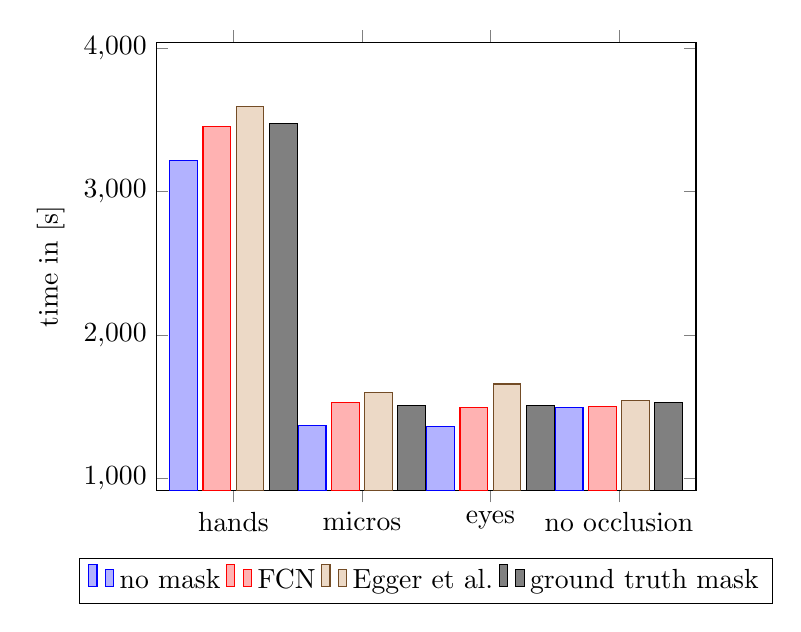
\begin{tikzpicture} 
		\begin{axis}[ 
		ybar, 
		enlargelimits=0.2, 
		legend style={at={(0.5,-0.15)}, anchor=north,legend columns=-1}, 
		ylabel={time in [s]}, 
		symbolic x coords={hands, micros, eyes, no occlusion}, 
		xtick=data, 
		%nodes near coords, 
		%nodes near coords align={vertical}, 
		] 
		
		\addplot coordinates {(hands,3220.89) (micros,1365.68) (eyes,1361.61) (no occlusion,1493.03)}; 
		\addplot coordinates {(hands,3457.30) (micros,1529.80) (eyes,1491.20) (no occlusion,1499.37)};
		\addplot coordinates {(hands,3597.28) (micros,1596.89) (eyes,1658.00) (no occlusion,1544.78)};
		\addplot coordinates {(hands,3476.42) (micros,1506.72) (eyes,1507.20) (no occlusion,1530.41)};
	
		
		\legend{no mask, FCN, Egger et al., ground truth mask} 
		\end{axis} 
		\end{tikzpicture}
	\end{center}
	\caption{Comparison of the Wall-Clock Time for the fitting process. The times were measured with the tailored 'face12' mask and the 'bfm' rendering.}
	\label{fig:chap3:times}
\end{figure}

Since we evaluated our experiments on a compute-server where we had no control of the priority of the process, we can't make a general statement about the absolute duration. Within a dataset all fits for the different segmentations were computed simultaneously. From this we can conclude that the fit with the FCN mask tends to require less time especially if the face is occluded by objects which can be recognized by the FCN.\\
\\
However, it is very difficult to make a general statement about the runtime behavior, because we cannot control whether the algorithm writes results in the cache and just loads them when desired, or computes them. As already mentioned, the Metropolis-Hastings algorithm proposes a randomly chosen face fit to be next one. If the evaluator rejects it, the algorithm uses the old fit as the next and just has to load it from the cache.  